\title{Lecture 3c: Policy Optimization}

% \author{Qi Zhang}
% \date{Last Updated: October 2025}

\section{The Policy Optimization Objective}
Value-based methods such as Q-learning maintain (only) value estimates as the RL agent's internal state and extract policies to finally recommend from those value estimates.
As the ultimate goal of RL is to find value-maximizing policies, in this note we consider a more direct approach, {\em policy optimization}, that, as its name suggests, directly maintains and optimizes a policy from experiences.

Formally, consider discounted-reward MDP $M=(\mathcal{S},\mathcal{A}, P, R, \gamma, d_0)$ where $d_0\in\Delta(\mathcal{S})$ is the initial state distribution, and let (in-episode) timesteps be 0-based indexed as $h=0,1,\ldots$ and $r_h:=R(s_h,a_h)$ be the reward at timestep $h$.
For policy $\pi:\mathcal{S}\to\Delta(\mathcal{A})$, its performance is quantified as $J(\pi)$, the expected discounted cumulative reward starting from an initial state $s_0 \sim d_0$ and follow policy $\pi$:
\begin{align*}
    J(\pi):= \E\left[\sum_{h=0}^{\infty} \gamma^h r_h ~\Big|~ s_0\sim d_0, a_h \sim \pi(s_h), s_{h+1}\sim P(s_h, a_h) \right]
    = \E_{s_0\sim d_0} \big[ V_\pi(s_0) \big]
    .
\end{align*}
The policy optimization problem is therefore
$
    \max_{\pi \in \Pi} J(\pi)
$, where $\Pi$ is a class of policies being searched over.
Policy optimization can be performed in the planning setting (i.e., MDP $M$ is fully known) or in the RL setting where the agent interacts with the MDP without requiring prior knowledge of $(P, R)$.

\section{Policy Gradient Methods: An Introduction}
\label{sec:Policy Gradient Methods: An Introduction}
For the rest of this note, we focus on the case where the policy class is parameterized as $\Pi=\{\pi_\theta: \theta\in\Theta\}$, where parameter space $\Theta\subseteq\R^n$ is a set of continuous real vectors.
Therefore, identifying a good policy in $\pi_\theta \in \Pi$ is equivalent to identifying a good parameter $\theta$.
We assume that $\pi_\theta(a|s)$ is differentiable with respect to $\theta$ for all $(s,a)\in\mathcal{S}\times\mathcal{A}$ and let $\nabla_\theta\pi_\theta(a|s)$ denote the derivative.

A good example to keep in mind is the {\em neural policy} where a neural network is parameterized by $\theta$, takes as input state $s$, and outputs $\pi_\theta(a|s)$ for all $a\in\mathcal{A}$, and therefore the differentiation of $\pi_\theta(a|s)$ can be achieved efficiently by backpropagation.

To search over such $\Pi$, we here consider gradient ascent methods that update parameter $\theta$ iteratively. 
For simplicity, we consider the unconstrained case where $\theta$ always remains in the valid set $\Theta$ after the update (e.g., $\Theta=\R^n$).
For example, the standard gradient ascent update is $\theta \gets \theta + \alpha \nabla_\theta J(\pi_\theta)$ where scalar $\alpha>0$ determines the size of the update in the direction of the {\em policy gradient}:
\begin{align}
\label{eq:PG_numerical}
   \nabla_\theta J(\pi_\theta)  = \left[\tfrac{\partial J(\pi_\theta)}{\partial\theta_1},\ldots,\tfrac{\partial J(\pi_\theta)}{\partial\theta_n}\right]\in\R^n,
   \quad\text{where }
   \tfrac{\partial J(\pi_\theta)}{\partial\theta_i}
   = \lim_{\Delta\theta_i \to 0} \frac{J(\pi_{\theta+\Delta\theta_i})-J(\pi_\theta)}{\Delta\theta_i}.
\end{align}

In principle, $\nabla_\theta J(\pi_\theta)$ can be numerically evaluated as in \eqref{eq:PG_numerical} by evaluating the policies before and after the $n$ small perturbations (), but it is impractical when $n$ is large.  
It turns out policy gradient $\nabla_\theta J(\pi_\theta)$ can be expressed in closed-form and there are even more than one such closed-form expression.

\subsection{REINFORCE}
We begin with the simplest policy gradient form called REINFORCE, which applies to the case where any episode always terminates after a finite number of $H$ transitions. We denote the trajectory of an episode and its cumulative discounted reward as 
\begin{align*}
    \tau = (s_0, a_0, r_0, \ldots, s_{H-1}, a_{H-1}, r_{H-1}, s_H),\quad
    R(\tau) = \textstyle \sum_{h=0}^{H-1}\gamma^hr_h
    .
\end{align*}
The probability of obtaining a particular trajectory $\tau$ when following policy $\pi$ is
\begin{align*}
    P^\pi(\tau) = d_0(s_0) \pi(a_0 | s_0) P\left(s_1 \mid s_0, a_0\right) \cdots \pi(a_{H-1} | s_{H-1})  P\left(s_{H} \mid s_{H-1}, a_{H-1}\right)
\end{align*}
For notation conciseness, we will drop the subscript $\theta$ in $\nabla_\theta$ and $\pi_\theta$.
The policy gradient can then be computed as 
\begin{align}
\nabla J(\pi) =&~ \nabla \E_{\tau\sim\pi}\left[R(\tau)\right] \nonumber\\
=&~ \nabla \left(\sum_{\tau} R(\tau) P^\pi(\tau)\right)\nonumber\\
=&~\sum_\tau R(\tau) \nabla P^\pi(\tau) \nonumber\\
=&~\sum_\tau R(\tau) P^\pi(\tau) \nabla \log P^\pi(\tau)  \qquad\text{\bf(Homework 2's 2a)}\nonumber\\
=&~\sum_\tau R(\tau) P^\pi(\tau) \nabla \log \Big(d_0(s_0) \pi(a_0 | s_0) P\left(s_1 \mid s_0, a_0\right) \cdots \pi(a_{H-1} | s_{H-1})\Big) \nonumber\\
=&~\sum_\tau R(\tau) P^\pi(\tau) \textstyle\nabla\left(\log d_0(s_0)+\sum_{h=0}^{H-1} \log \pi(a_h | s_h)+\sum_{h=0}^{H-1} \log P\left(s_{h+1} \mid s_h, a_h\right)\right) \nonumber\\
=&~\sum_\tau R(\tau) P^\pi(\tau) \textstyle\nabla\left(\sum_{h=0}^{H-1} \log \pi(a_h | s_h)\right)
\qquad\text{\bf(Homework 2's 2b)}
\label{eq:PG_REINFORCE}\\ 
=&~\mathbb{E}_{\tau \sim \pi}\Big[\underbrace{R(\tau) \textstyle\sum_{h=0}^{H-1} \nabla \log \pi(a_h | s_h)}_{\widehat{g}^{\text{ REINFORCE-1}}(\tau)}\Big]
\label{eq:REINFORCE-1}
.
\end{align}
We now discuss how to utilize the derivations above:
\begin{itemize}
    \item In the planning setting where MDP $M$ is fully known, we can compute $P^\pi(\tau)$ for any trajectory $\tau$.
    Therefore, we can enumerate all possible trajectories to compute $\nabla J(\pi)$ exactly via \eqref{eq:PG_REINFORCE}. 
    \item In the RL setting, $(P,R)$ is unknown and therefore we cannot compute $P^\pi(\tau)$ or \eqref{eq:PG_REINFORCE}.
    Instead, the estimator $\widehat{g}^{\text{ REINFORCE-1}}(\tau)$ as defined in \eqref{eq:REINFORCE-1} is an unbiased estimator of $\nabla J(\pi)$ and we can update the parameter in a stochastic gradient ascent fashion, e.g. $\theta \gets \theta + \alpha \widehat{g}(\tau)$, with trajectory $\tau$ sampled from current policy $\pi=\pi_\theta$.
    The resulting RL algorithm, REINFORCE, is outlined in Algorithm \ref{algorithm:REINFORCE}.
\end{itemize}
\begin{algorithm}
\caption{REINFORCE} \label{algorithm:REINFORCE}
\begin{algorithmic}[1]
\State {learner initializes parameter $\theta$ for policy $\pi_\theta$;}
\Repeat {~over episodes:}
    \State learner finishes current episode $\tau$ by following $\pi_\theta$ until termination; 
    \State learner updates parameter $\theta$ with REINFORCE estimator $\widehat{g}(\tau)$ (cf. \eqref{eq:REINFORCE-1} \eqref{eq:REINFORCE-2});
\Until{some stopping criterion is met}
\State learner outputs policy $\widehat{\pi} =\pi_\theta$ or $\widehat{\pi}(s) =\argmax_{a\in\mathcal{A}}\pi_\theta(a|s)$;
\label{algorithm:RL interaction:line:final policy}
\end{algorithmic}
\end{algorithm}


\subsection{The action-value expression}
Although the gradient estimator of \eqref{eq:REINFORCE-1} is unbiased, it is often of high variance, which will then hurt the performance of the stochastic gradient ascent.
We next derive alternative policy gradient estimators that usually are of lower variances.
A thorough discussion of variance reduction techniques for policy gradient is beyond the scope of this note.

One reason that estimator \eqref{eq:REINFORCE-1} is of high variance is due to the episodic reward $R(\tau)$: its summation of rewards over many steps is usually of high variance.
This issue can be alleviated by turning to an alternative expression of policy gradient that essentially replace the episodic reward with the action-values:
\begin{align}
\label{eq:PG_Qvalue}
    \nabla J(\pi) = \E_{(s,a)\sim d^\pi}\left[\nabla\log\pi(a|s)\cdot Q^\pi(s,a)\right]
\end{align}
Here, $d^\pi$ is the (unnormalized) state-action {\em occupancy measure} that accumulates the discounted expectation of visitation of state-action pairs over time:
\begin{align*}
    d^\pi(s,a):=\sum_{h=0}^{\infty}\gamma^t d_h^\pi(s,a)
    \text{ with }
    d_h^\pi(s,a):=\Pr(s_h=s, a_h=a \mid s_0\sim d_0, \pi).
\end{align*}
Here, $d^\pi(s,a)$ is not a probability measure (i.e., $\sum_{(s,a)}d^\pi(s,a) \neq 1$), but we still interpret the expectation as $\E_{(s,a)\sim d^\pi}[\cdot] = \sum_{s,a}d^\pi(s,a)(\cdot)$.

Again, in the planning setting, $d^\pi$ and $Q^\pi$ can be exactly computed, and therefore policy gradient $\nabla J(\pi)$ can be exactly computed via \eqref{eq:PG_Qvalue}.
To see how \eqref{eq:PG_Qvalue} yields a gradient estimator for the RL setting, note the following fact: 
for any function $f(s,a)$ on state-action pairs, 
\begin{align}
\label{eq:occupancy_property}
    \E_{(s,a)\sim d^\pi}[f(s,a)] = \E_{\tau\sim\pi}\left[\sum_{h=0}^\infty \gamma^h f(s_h,a_h)\right].
\end{align}
We omit a proof of \eqref{eq:occupancy_property}, but it is fairly intuitive:
$d^\pi$ accumulates discounted visitation of state-action pair $(s,a)$ by following $\pi$, so it is equivalent to using $\pi$ to sample trajectories and averaging over timesteps.
From this, we can obtain another policy gradient estimator:
\begin{align}
    \nabla J(\pi) =&~ \E_{(s,a)\sim d^\pi}\left[\nabla\log\pi(a|s)\cdot Q^\pi(s,a)\right] \nonumber\\
    =&~\E_{\tau\sim\pi}\left[\textstyle\sum_{h=0}^{H}\gamma^h \nabla\log\pi(a_h|s_h)\cdot Q^\pi(s_h,a_h)\right] && \text{($\tau$ terminates after $H$ transitions)}\nonumber\\
    =&~\E_{\tau\sim\pi}\Big[\underbrace{\textstyle\sum_{h=0}^{H}\gamma^h \nabla\log\pi(a_h|s_h)\cdot \sum_{h'=h}^H \gamma^{h'-h} r_{h'}}_{{\widehat{g}^{\text{REINFORCE-2}}(\tau)}}\Big] \label{eq:REINFORCE-2}
\end{align}
Roughly speaking, the last equality above is due to $\E_{\tau\sim\pi}[Q^\pi(s_h,a_h)] = \E_{\tau\sim\pi}[\sum_{h'=h}^H \gamma^{h'-h} r_{h'}]$, and a more rigorous argument can be made via law of total expectation (conditioned on particular realizations of $(s_h,a_h)$).
The resulting estimator $\widehat{g}^{\text{REINFORCE-2}}(\tau)$ in \eqref{eq:REINFORCE-2} can then be used as the gradient estimator in Algorithm \ref{algorithm:REINFORCE}.

\section{Policy Optimization in a Trust Region, Proximal Policy Optimization}
All methods in Section \ref{sec:Policy Gradient Methods: An Introduction}, often referred to as {\em vanilla policy gradient} methods, adopt the standard gradient ascent approach that updates the parameter with a single step aligned with the policy gradient, with different methods varying in how the gradient estimation is performed.
In this section, we introduce another family of methods, {\em trust region} policy optimization methods, that update the current policy parameter with multiple gradient steps.
We will describe in detail one such method, Proximal Policy Optimization (PPO),
which is easy to implement and are in many cases more efficient and stable than vanilla policy gradient methods.

\subsection{Policy optimization in a trust region.}
The key idea behind the trust region methods is to form a surrogate objective that well approximates the true objective to $J(\pi_\theta)$ within a local region, i.e., trust region, where the deviation from $\pi_\theta$ is sufficiently small.
The technical tool to form such a surrogate objective is the {\em Performance Difference Lemma} that quantifies the difference in the values of two policies:
\begin{lemma}
[Performance Difference Lemma]
\label{lemma:Performance Difference Lemma}
For any two policies $\pi, \pi'$,
\begin{align*}
    J(\pi') - J(\pi) = \E_{{(s,a)}\sim d^{\pi'}}\left[A^\pi(s,a)\right]
\end{align*}
where $A^\pi(s,a):= Q^\pi(s,a)-V^\pi(s)$ is called the advantage of policy $\pi$.
\end{lemma}
To use Lemma \ref{lemma:Performance Difference Lemma} to optimize $J(\pi_\theta)$, consider setting $\pi=\pi_{\theta_{\text{old}}}$ and $\pi'=\pi_\theta$,
where $\theta_{\text{old}}$ is the parameter of the current policy from which we have sampled trajectories ($\tau\sim\pi_{\theta_{\text{old}}}$) and $\theta$ is the candidate policy parameter we are optimizing over.
We proceed as 
\begin{align*}
    J(\pi_\theta) - J(\pi_{\theta_{\text{old}}})=&~ \E_{(s,a)\sim d^{\pi_\theta}}\left[A^{\pi_{\theta_{\text{old}}}}(s,a)\right]\\
    =&~\E_{s\sim d^{\pi_\theta},~ a\sim\pi_\theta(s)}\left[A^{\pi_{\theta_{\text{old}}}}(s,a)\right]
    ~~\text{($d^{\pi_\theta}$ is abused as the marginal state distribution)}\\
    =&~\E_{s\sim d^{\pi_\theta},~ a\sim\pi_{\theta_{\text{old}}}(s)}\left[\frac{\pi_\theta(a|s)}{\pi_{\theta_{\text{old}}}(a|s)}A^{\pi_{\theta_{\text{old}}}}(s,a)\right] \qquad\text{\bf(Homework 2's 2c)} \\
    \approx&~\E_{s\sim d^{\pi_{\theta_{\text{old}}}},~ a\sim\pi_{\theta_{\text{old}}}(s)}\left[\frac{\pi_\theta(a|s)}{\pi_{\theta_{\text{old}}}(a|s)}A^{\pi_{\theta_{\text{old}}}}(s,a)\right]\\
    =&~ \E_{(s,a)\sim d^{\pi_{\theta_{\text{old}}}}}\left[\frac{\pi_\theta(a|s)}{\pi_{\theta_{\text{old}}}(a|s)}A^{\pi_{\theta_{\text{old}}}}(s,a)\right] =: L(\theta)
\end{align*}
The above derivation is useful because:
\begin{itemize}
    \item Since $\pi_{\theta_{\text{old}}}$ is fixed, $\max_\theta J(\theta)$ is equivalent to $\max_\theta (J(\pi_\theta)-J(\pi_{\theta_{\text{old}}}))$, i.e., maximizing the improvement of $\pi_\theta$ over $\pi_{\theta_{\text{old}}}$, which is exactly what is being quantified.
    \item According to the first equality, the exact improvement can be estimated by trajectories sampled from $\pi_\theta$ (i.e., $\E_{d^{\pi_\theta}}$) but we only have trajectories from $\pi_{\theta_{\text{old}}}$.
    To solve this issue, the derivation replaces $d^{\pi_\theta}$ with $d^{\pi_{\theta_{\text{old}}}}$, using the importance sampling trick (the third equality) and also paying the approximation error ($\approx$).
    In the RL setting, we can approximate $\E_{(s,a)\sim d^{\pi_{\theta_{\text{old}}}}}$ via trajectories sampled from the policy, $\tau\sim\pi_{\theta_{\text{old}}}$, as justified in Equation \eqref{eq:occupancy_property}.
    These trajectories can also be used to estimate advantages $A^{\pi_{\text{old}}}$.
    \item  The approximation, $L(\theta)$, is the surrogate objective we will be optimizing, which is a good approximation when $\pi_{\theta}$ is not too different from $\pi_{\theta_{\text{old}}}$ (so $d^{\pi_{\theta}}$ is not too different from $d^{\pi_{\theta_{\text{old}}}}$):
    \begin{align}
    \label{eq:trust_region}
        \max_{\theta}~ L(\theta)\quad \text{subject to: $\pi_{\theta}$ is not too different from $\pi_{\theta_{\text{old}}}$}
    \end{align}

    \item We can perform a full-scale optimization of \eqref{eq:trust_region}, e.g., via multiple gradient ascent steps. After the optimization, we will set $\theta_{\text{old}}$ to the solution and iteratively proceed to the next round.
\end{itemize}

\subsection{PPO}
PPO is an easy-to-implement method for the optimization problem of \eqref{eq:trust_region}.
Instead of a hard-coded trust region constraint, PPO performs the unconstrained optimization of a clipped version of $L(\theta)$:
letting $r_\theta(a|s):=\frac{\pi_\theta(a|s)}{\pi_{\theta_{\text{old}}}(a|s)}$
\begin{align*}
    \max_\theta~
    \E_{(s,a)\sim d^{\pi_{\theta_{\text{old}}}}}\Big[\min\Big\{
    \underbrace{r_\theta(a|s)A^{\pi_{\theta_{\text{old}}}}(s,a)}_{\text{same as in $L(\theta)$}},\quad
    \underbrace{\operatorname{clip}^{1+\epsilon}_{1-\epsilon}\big(r_\theta(a|s)\big)A^{\pi_{\theta_{\text{old}}}}(s,a)}_{\text{same, but with $r_\theta$ clipped}}
    \Big\}\Big].
\end{align*}
The clipping implicitly discourages changing $\pi_\theta$ too much from $\pi_{\theta_{\text{old}}}$.
Figure \ref{fig:ppo} illustrates what would happen respectively for advantage being positive vs negative and the policy ratio being clipped vs not clipped.
\begin{figure}[htb]
\centering
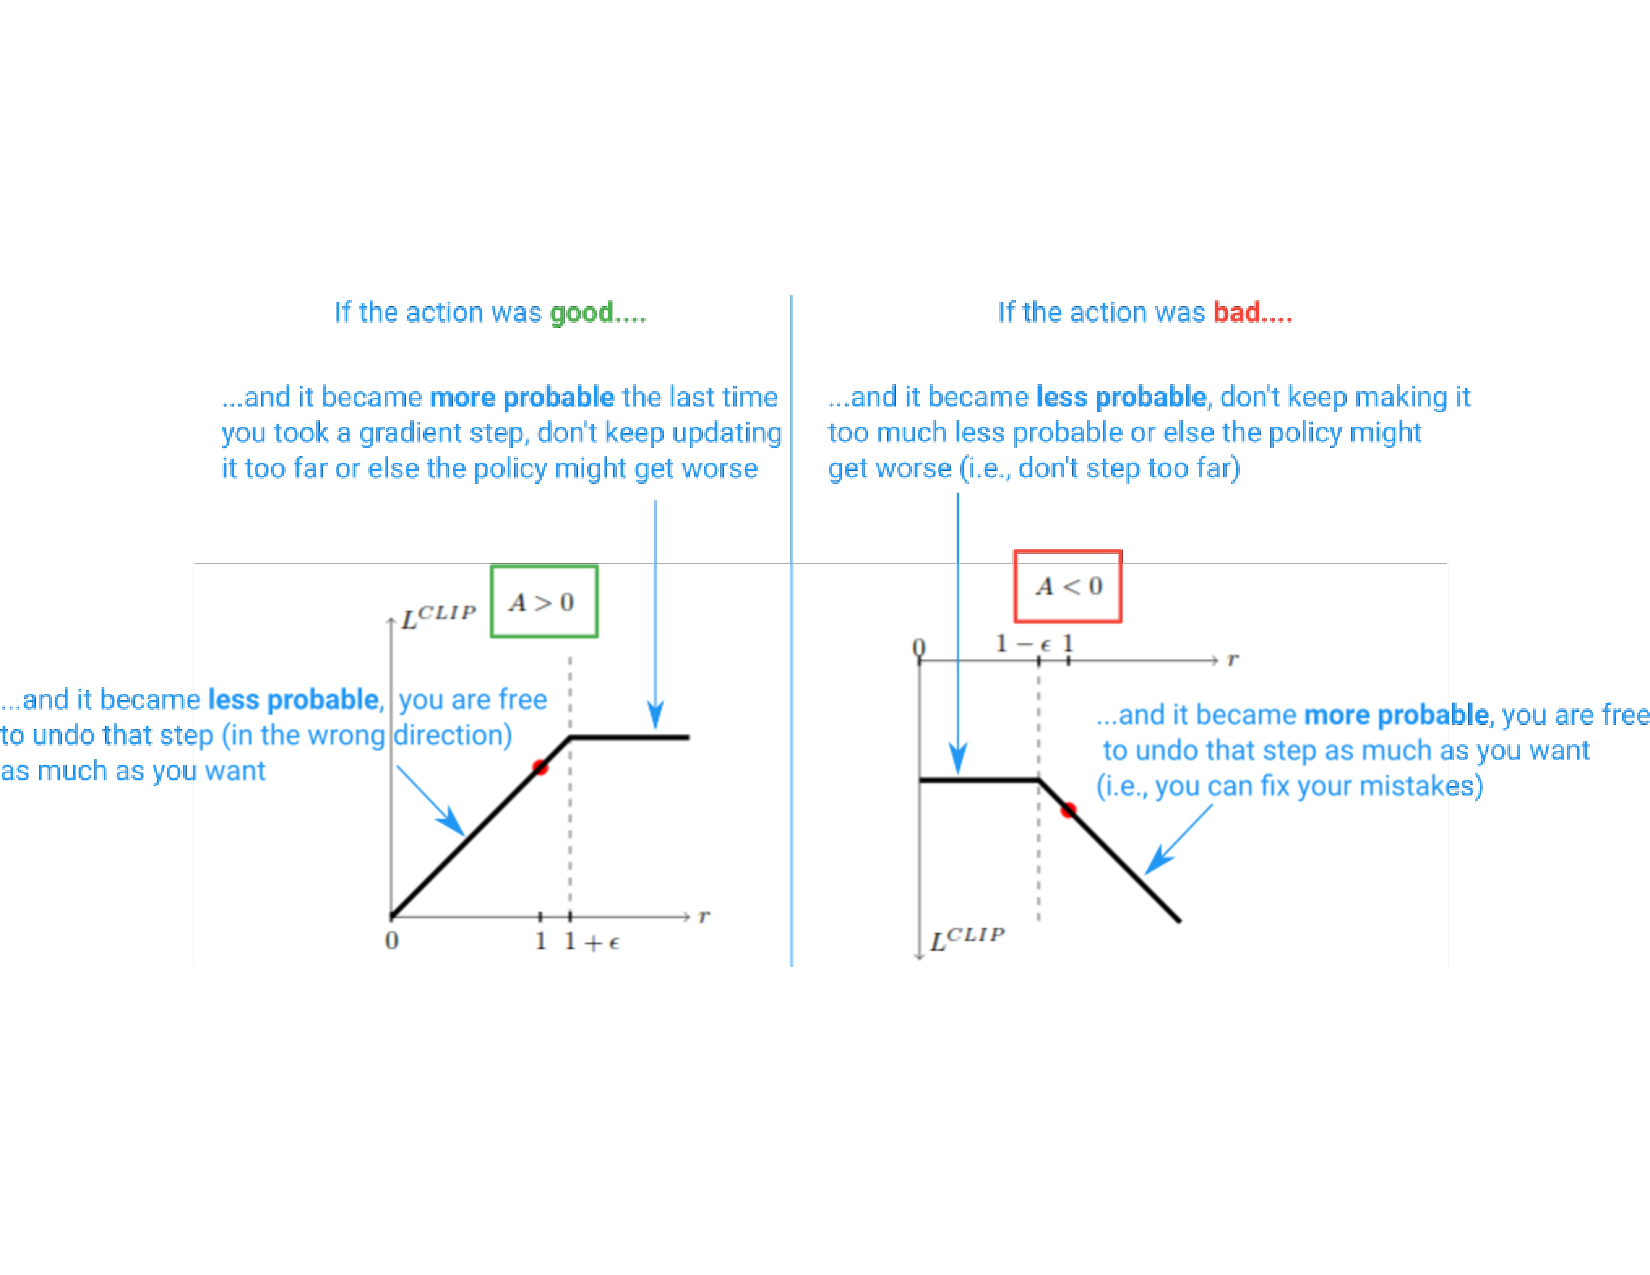
\includegraphics[width=1.\textwidth]{lectures/figures/gasbI.pdf}
\caption{
Plot showing one term for a certain $(s,a)$-pair of the PPO objective as a function of the policy ratio $r_\theta(a|s)$.
Credit to
\href{https://stackoverflow.com/questions/46422845/what-is-the-way-to-understand-proximal-policy-optimization-algorithm-in-rl}{this post}.
}
\label{fig:ppo}
\end{figure}



\paragraph{Implementation details.}
We provide a pseudocode of PPO in Algorithm \ref{algorithm:PPO}, which should be useful for you to implement it in hw3.ipynb.
The PPO version you will implement in hw3.ipynb is significantly simplified from a standard version, particularly on 1) how the policy is parameterized and how 2) the advantages are estimated (line \ref{algorithm:PPO: line:advantage}).
We recommend a standard PPO implementation (like \href{https://github.com/vwxyzjn/cleanrl}{this one}) for regular use cases.
\begin{algorithm}
\caption{Proximal Policy Optimization (PPO) with clipped objective} \label{algorithm:PPO}
\begin{algorithmic}[1]
\State learner initializes parameter $\theta$ for policy $\pi_\theta$;
\State $\theta_{\text{old}}\gets\theta$;
\Repeat
    \State Follow $\pi_{\theta_{\text{old}}}$ to collect and store multiple transitions $\{(s_t,a_t,r_t,s_{t+1})\}$;
    \State Estimates advantages $\widehat{A}_t\approx A^{\pi_{\theta_{\text{old}}}}(s_t,a_t)$;
    \Comment{Can involve training and using a {\em critic}}
    \label{algorithm:PPO: line:advantage}
    \State Optimize $\theta$ to maximize
    \begin{align*}
        &\qquad\quad\E_{t}\Big[\min\big\{
    r_t(\theta) \widehat{A}_t,~
    \operatorname{clip}^{1+\epsilon}_{1-\epsilon}\big(r_t(\theta)\big)\widehat{A}_t
    \big\}\Big]\\
    &\text{where $r_t(\theta):= \tfrac{\pi_\theta(a_t|s_t)}{\pi_{\theta_{\text{old}}}(a_t|s_t)}$ and $\E_{t}$ denotes sampling from the stored transitions;}
    \end{align*}
    \State Update parameter $\theta_{\text{old}}\gets\theta$;
\Until{some stopping criterion is met}
\State learner outputs policy $\widehat{\pi} =\pi_\theta$ or $\widehat{\pi}(s) =\argmax_{a\in\mathcal{A}}\pi_\theta(a|s)$ with $\theta = \theta_{\text{old}}$;
\label{algorithm:RL interaction:line:final policy}
\end{algorithmic}
\end{algorithm}



